\documentclass[12pt]{article}
\usepackage[utf8]{inputenc}
\usepackage{graphicx}
\usepackage{float}
\usepackage{hyperref}
\usepackage{booktabs}
\usepackage{geometry}
\geometry{margin=1in}

\title{Final Report: Reinforcement Learning with Pre-Collected Datasets (RLPD) and SAC}
\author{Tara Denaud Joseph, Richa Kewalramani, and Fay Lee}
\date{December 19, 2025}

\begin{document}

\maketitle

\begin{abstract}
This report presents experiments on reinforcement learning with pre-collected datasets (RLPD) using the Soft Actor-Critic (SAC) algorithm. We evaluate Hopper-v4 and Ant-v5 environments, analyzing the effect of buffer size, batch size, and random seed on learning performance. AntMaze and Walker2d results are placeholders. An appendix contains references and further resources.
\end{abstract}

\section{Introduction}
Reinforcement learning (RL) is a paradigm in which agents learn to make decisions by interacting with an environment and receiving feedback in the form of rewards. While RL has achieved impressive results in many domains, traditional RL methods are often data inefficient: learning from scratch requires many environment interactions, which can be expensive or slow.

To address this limitation, we explore RL with pre-collected datasets (RLPD). By using pre-existing experience in a replay buffer, agents can bootstrap learning, reduce variance, and achieve better performance in fewer steps. This project focuses on applying Soft Actor-Critic (SAC), a popular off-policy RL algorithm, and comparing standard SAC with SAC trained using pre-collected data.

Recent work by Ball et al. (2023) demonstrates that standard off-policy RL methods can effectively leverage offline trajectories with minimal modifications, achieving up to a 2.5× improvement in online learning efficiency across various benchmarks. The authors also released the code publicly \cite{rlpd_github}, which guided our project.

\section{Methodology}

\subsection{Environments}
Experiments were conducted on the following continuous control environments:

\begin{itemize}
    \item \textbf{Hopper-v4:} A single-legged hopping agent.
    \item \textbf{Ant-v5:} A quadruped locomotion agent.
    \item \textbf{AntMaze:} Placeholder for a navigation task with goal-directed exploration.
    \item \textbf{Walker2d:} Placeholder for a two-legged walking agent.
\end{itemize}

\subsection{SAC Training}
SAC was implemented from scratch (\texttt{train\_baseline\_sac.py}) and trained with pre-collected data (\texttt{train\_with\_prior\_data.py}). Key steps included:

\begin{itemize}
    \item Initializing the environment and SAC agent.
    \item Training over a specified number of steps.
    \item Saving checkpoints at multiple intervals for later analysis.
\end{itemize}

For RLPD experiments, rollouts from partially trained SAC agents were collected (\texttt{collect\_from\_checkpoint.py}) and preloaded into the replay buffer. This allows the agent to learn from prior experience rather than relying purely on online interactions.

\subsection{Hyperparameters}
Key hyperparameters used in experiments:

\begin{table}[H]
\centering
\begin{tabular}{l l l}
\toprule
Parameter & Description & Typical Values \\
\midrule
buffer\_size & Replay buffer capacity & 50k -- 500k \\
batch\_size & Mini-batch size for updates & 64 -- 512 \\
learning\_rate & Optimizer step size & 3e-4 \\
seed & Random seed for reproducibility & 0 -- 4 \\
total\_steps & Number of environment interactions & 200k \\
\bottomrule
\end{tabular}
\caption{Hyperparameters used in SAC training.}
\end{table}

\section{Evaluation Methodology}
Experiments were evaluated across multiple seeds and checkpoints:

\begin{itemize}
    \item Seeds: 3 seeds for both Hopper-v4 and Ant-v5.
    \item Checkpoint evaluation: Metrics such as average reward and standard deviation were logged for each seed and checkpoint (\texttt{evaluation\_results.csv}).
    \item Visualization: Plots were generated for learning curves, buffer-size and batch-size comparisons, and seed variance (\texttt{plot\_results.py}, \texttt{plot\_seed\_variance.py}).
\end{itemize}

\section{Results and Outcomes}

\subsection{Hopper-v4}

\textbf{Buffer Size Comparison:}

\begin{figure}[H]
\centering
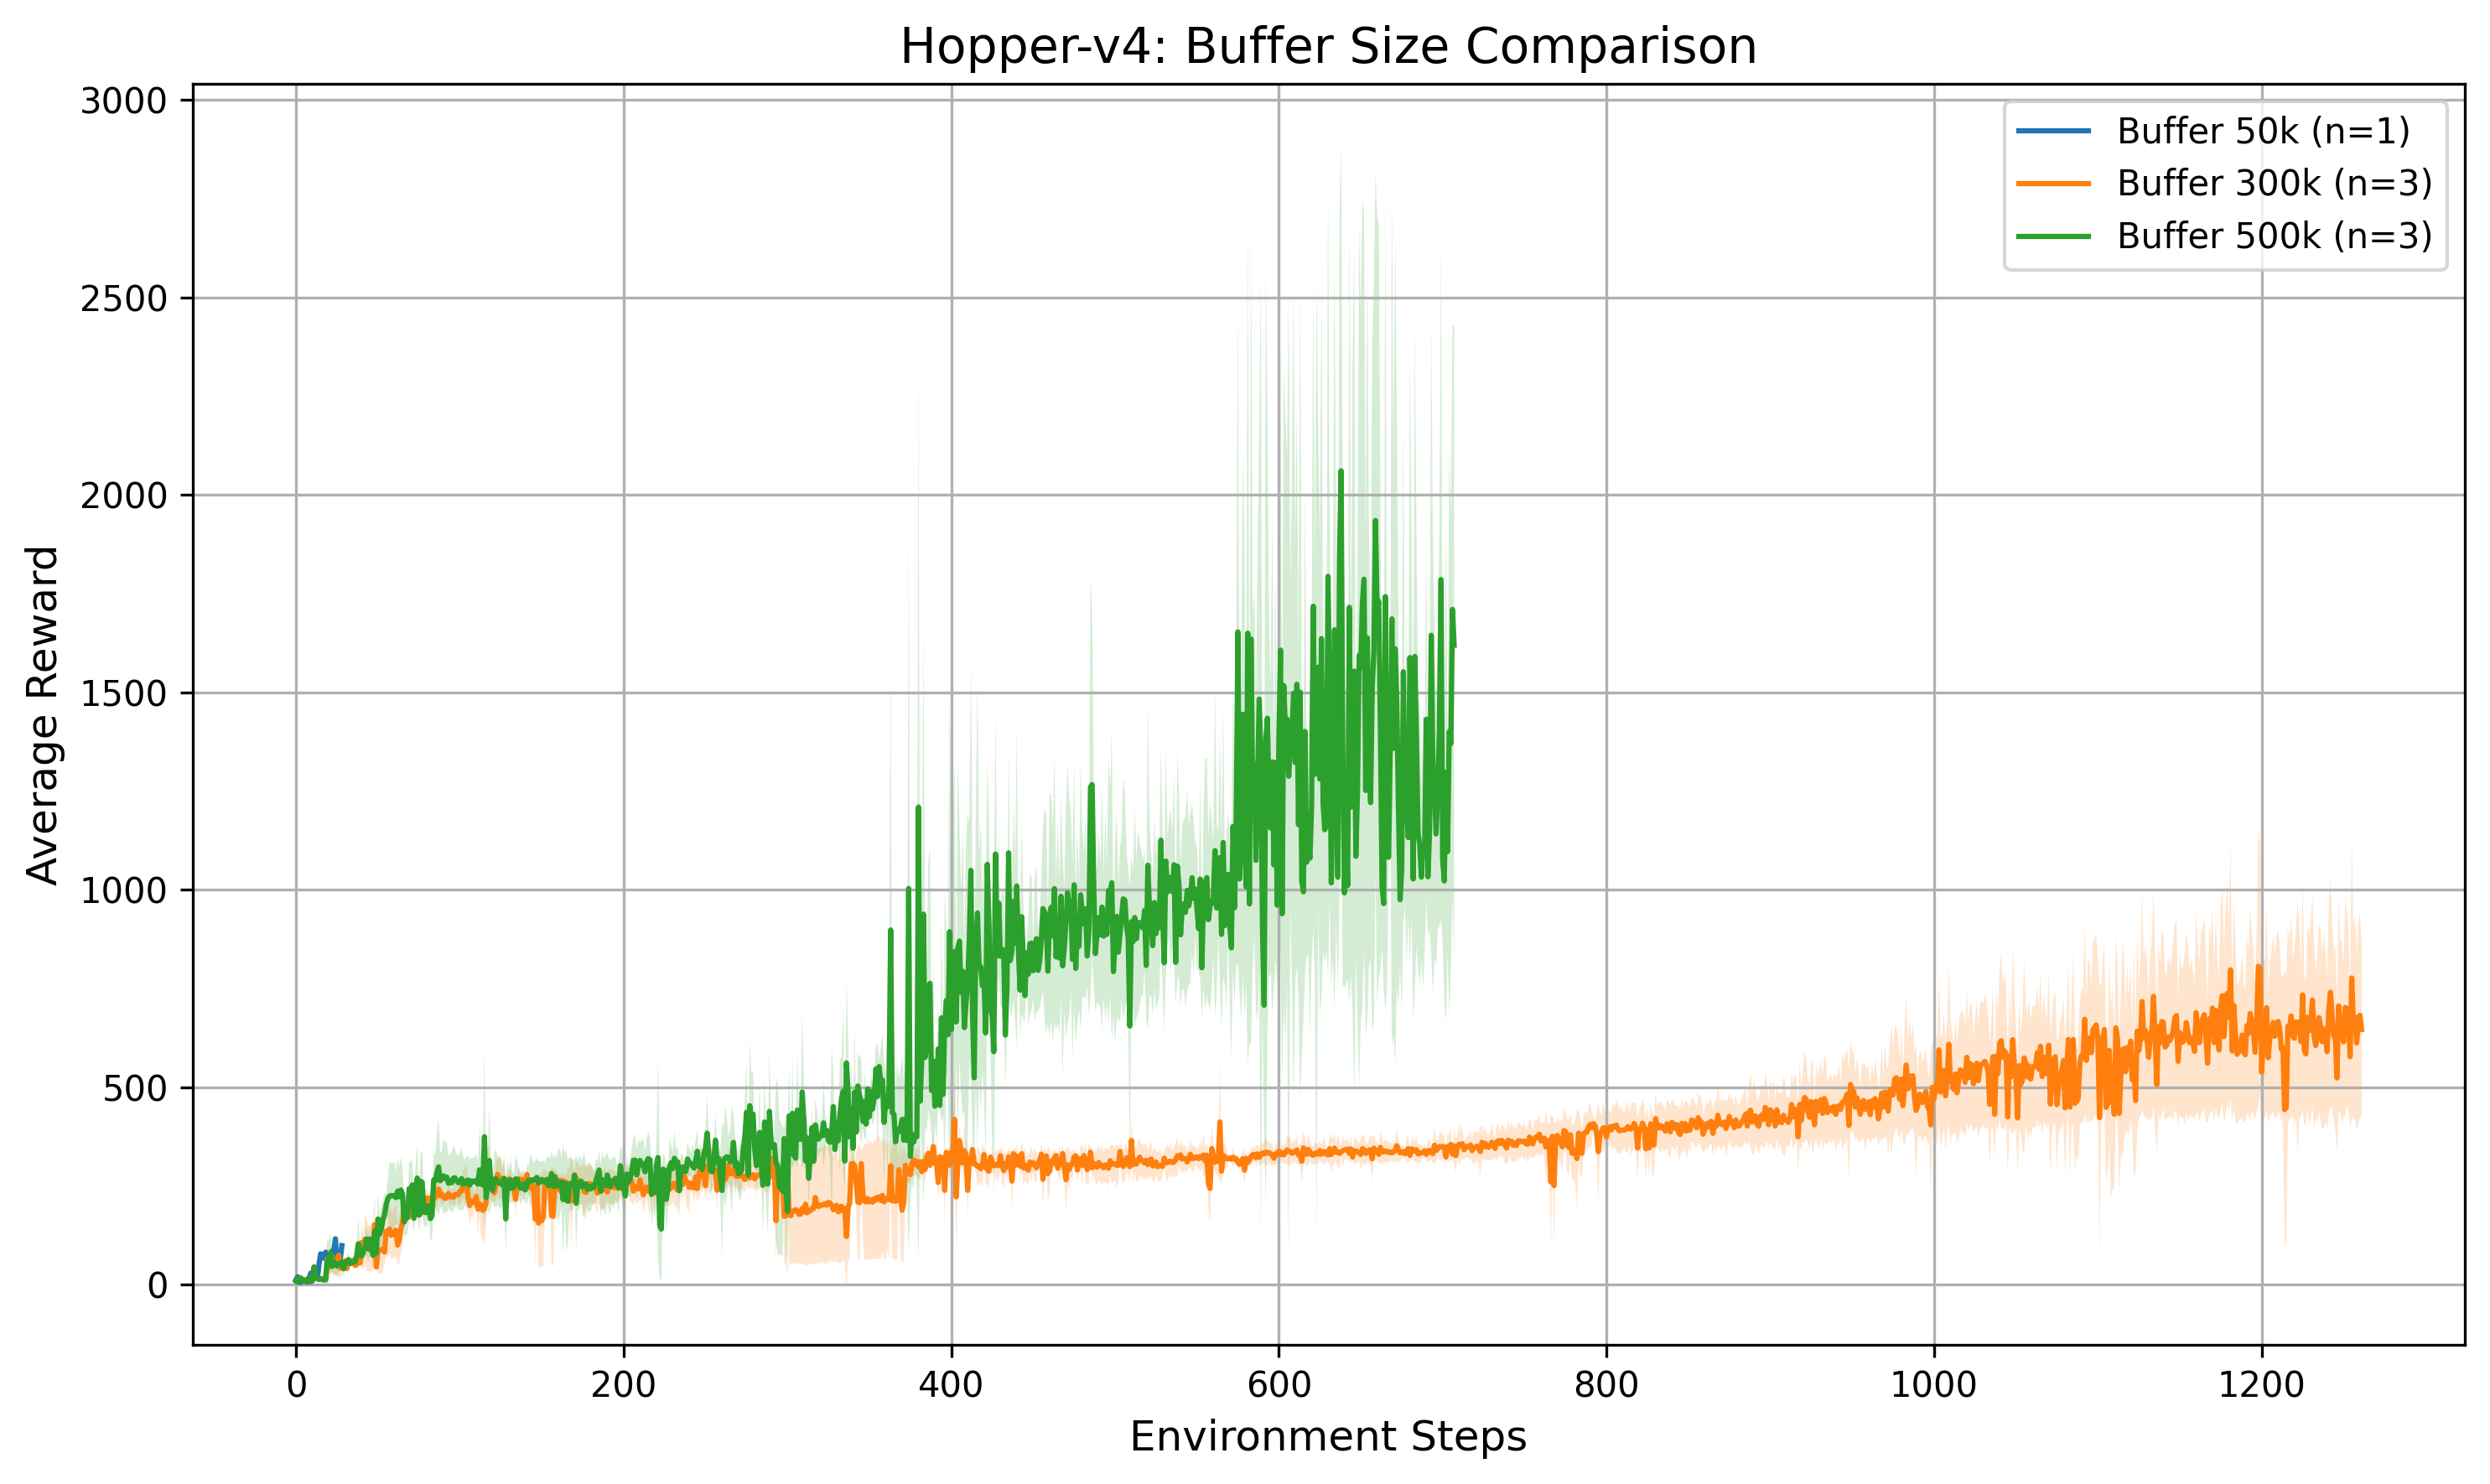
\includegraphics[width=0.7\textwidth]{figures/hopper_buffer_comparison.png}
\caption{Learning curves for Hopper-v4 with varying buffer sizes (n=3 seeds).}
\end{figure}

\textbf{Batch Size Comparison:}

\begin{figure}[H]
\centering
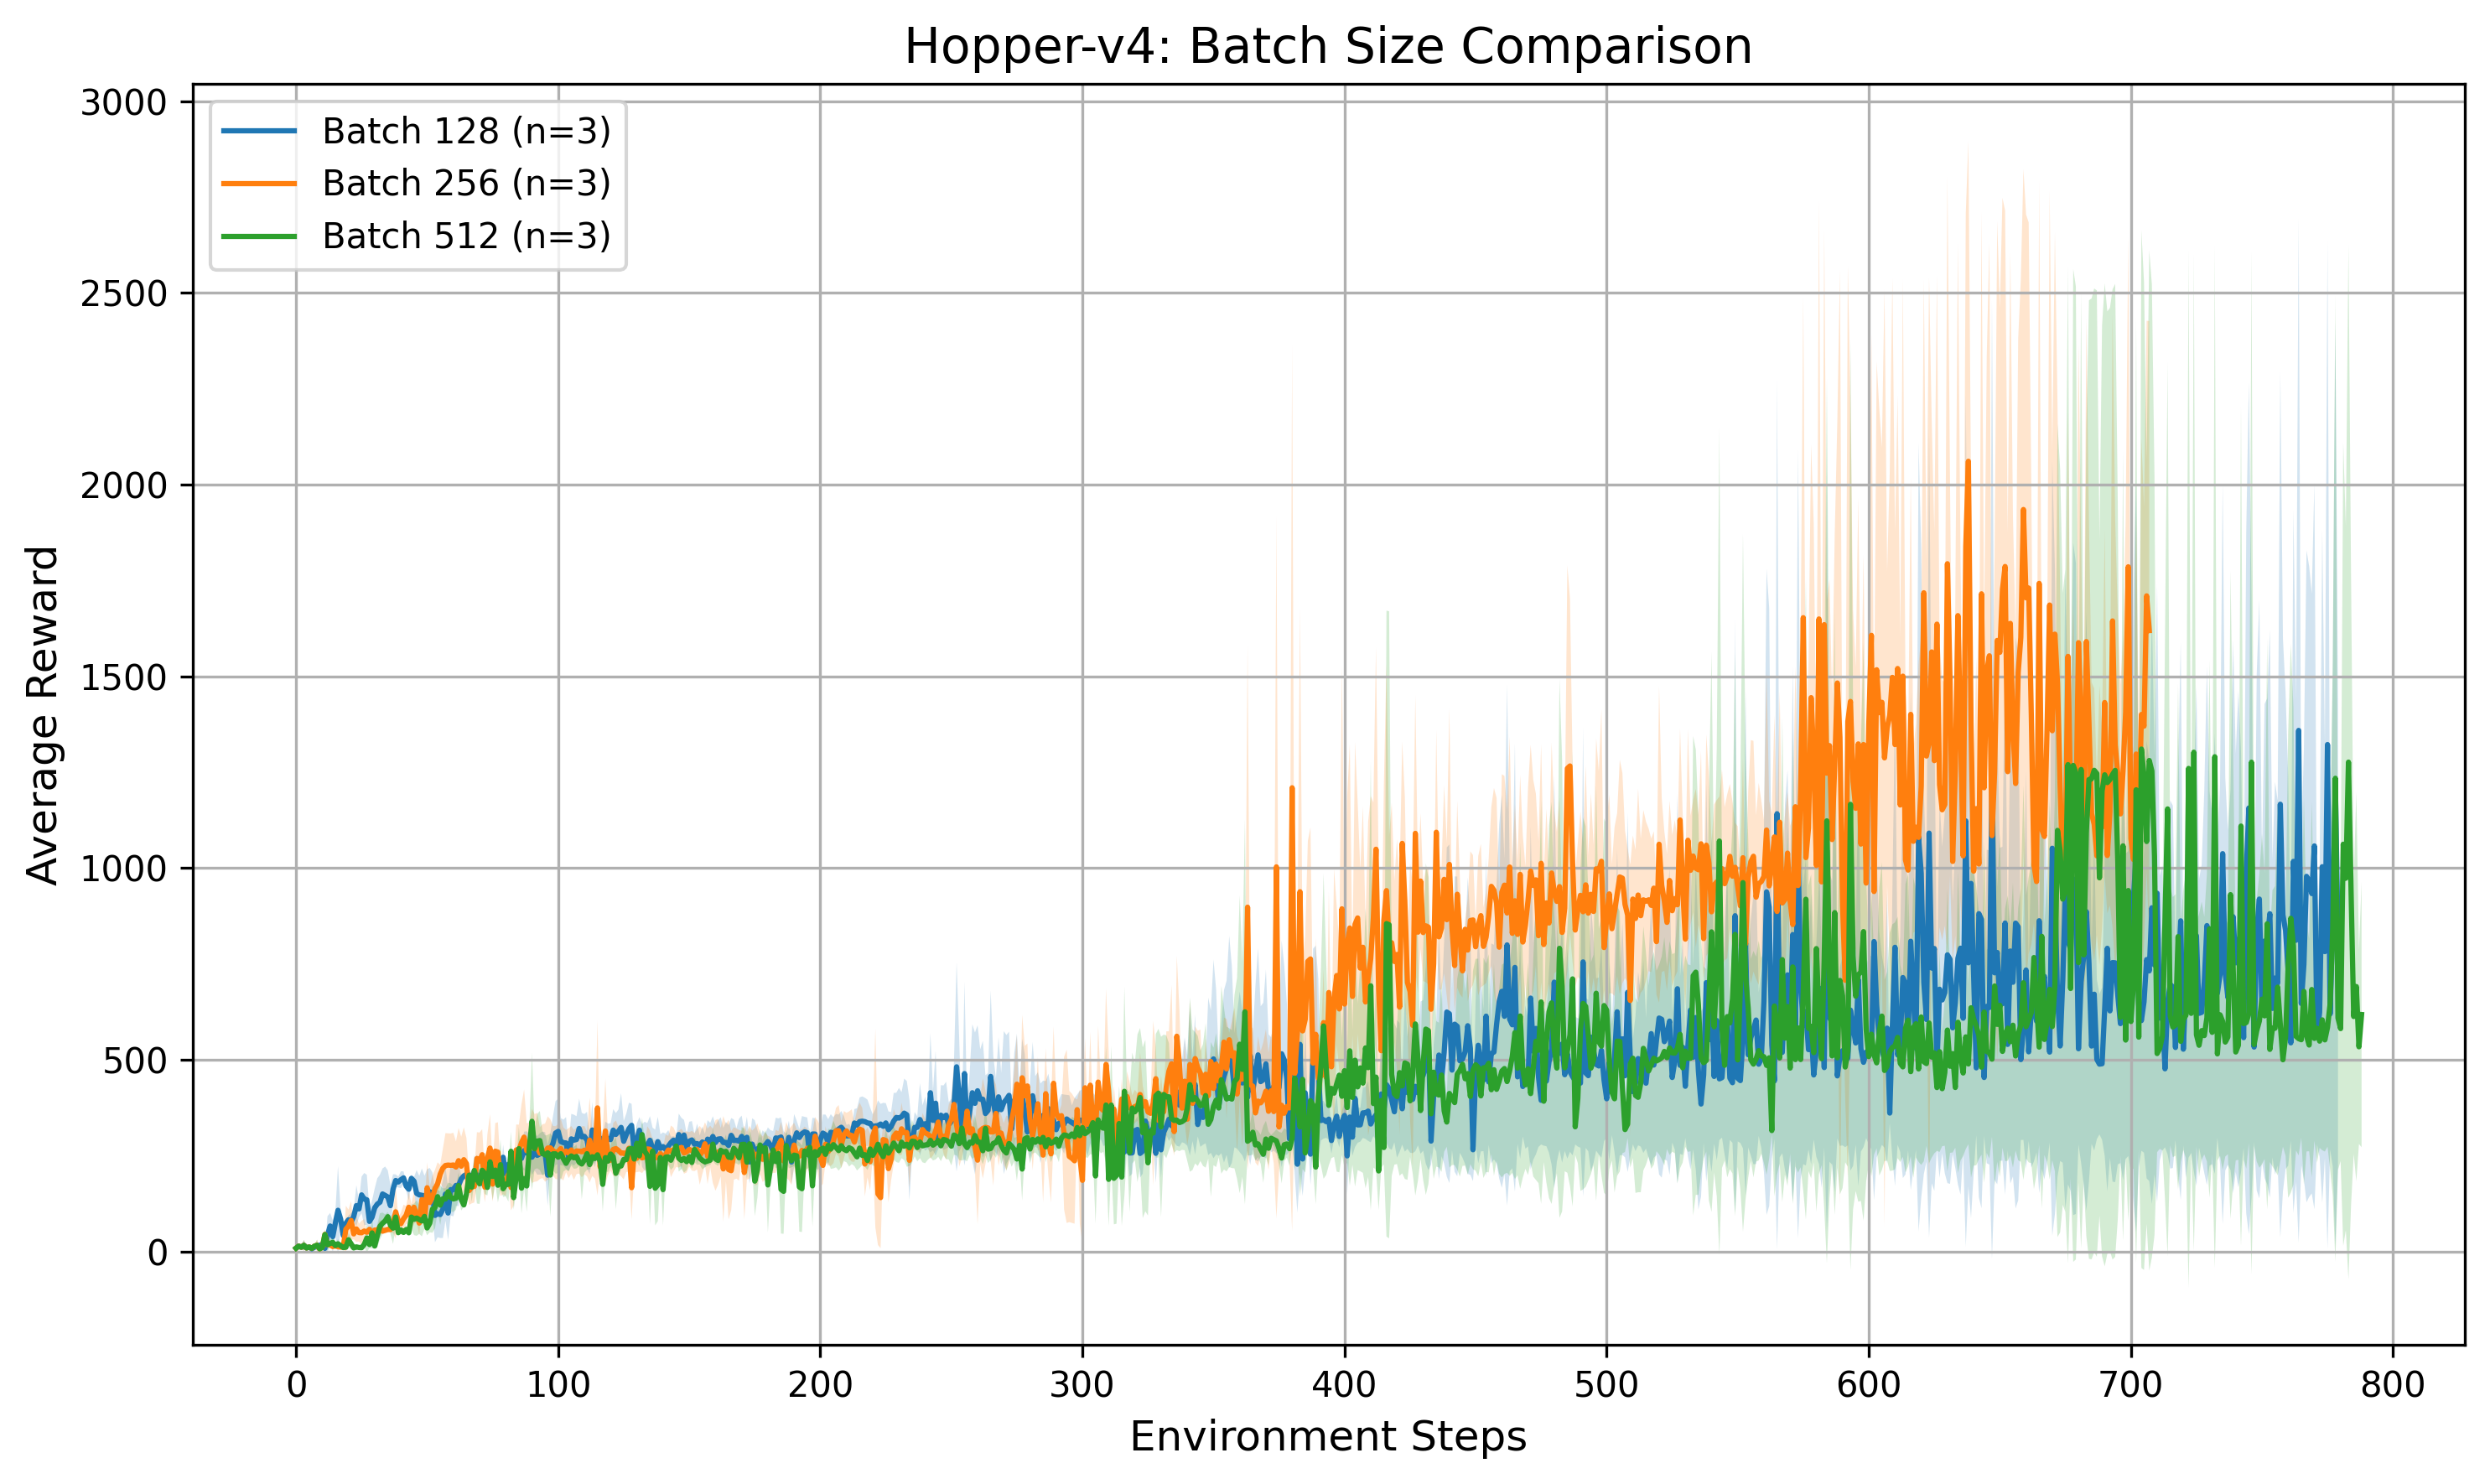
\includegraphics[width=0.7\textwidth]{figures/hopper_batch_comparison.png}
\caption{Learning curves for Hopper-v4 with varying batch sizes (n=3 seeds).}
\end{figure}

\textbf{Seed Variation:}

\begin{figure}[H]
\centering
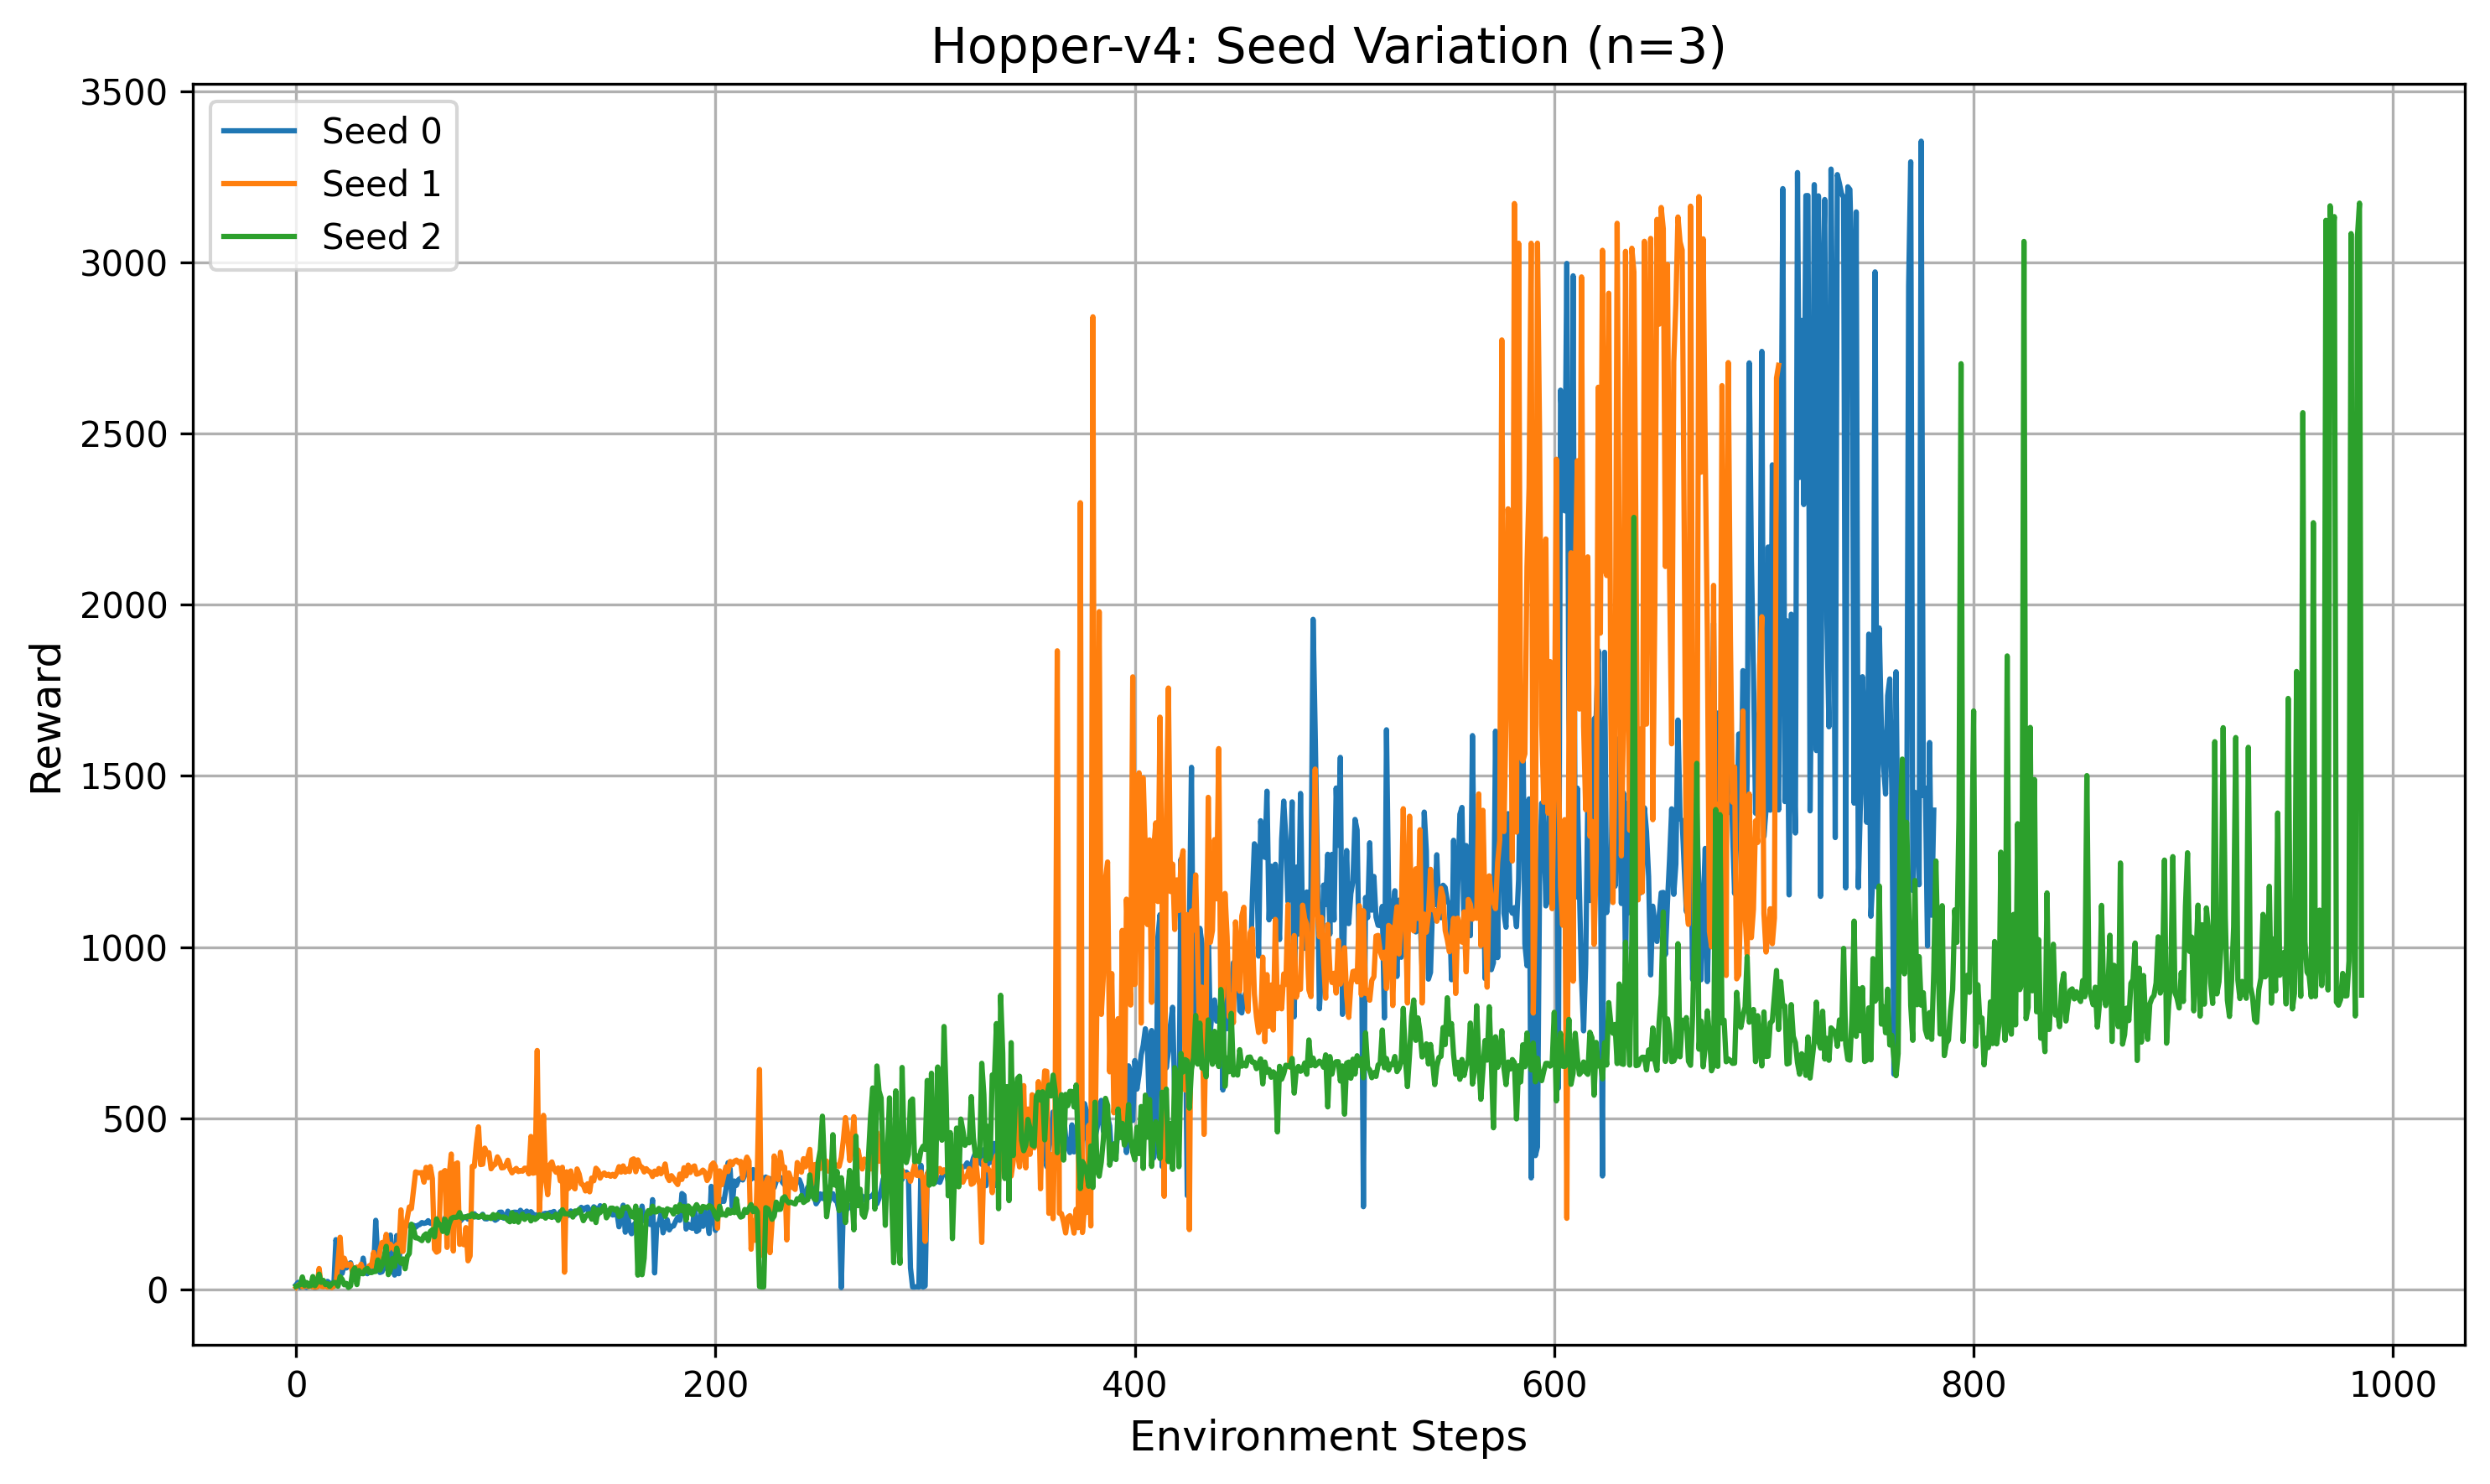
\includegraphics[width=0.7\textwidth]{figures/hopper_seed_variance.png}
\caption{Seed variation for Hopper-v4 across multiple runs (n=3 seeds).}
\end{figure}

\subsection{Ant-v5}

\textbf{Buffer Size Comparison:}

\begin{figure}[H]
\centering
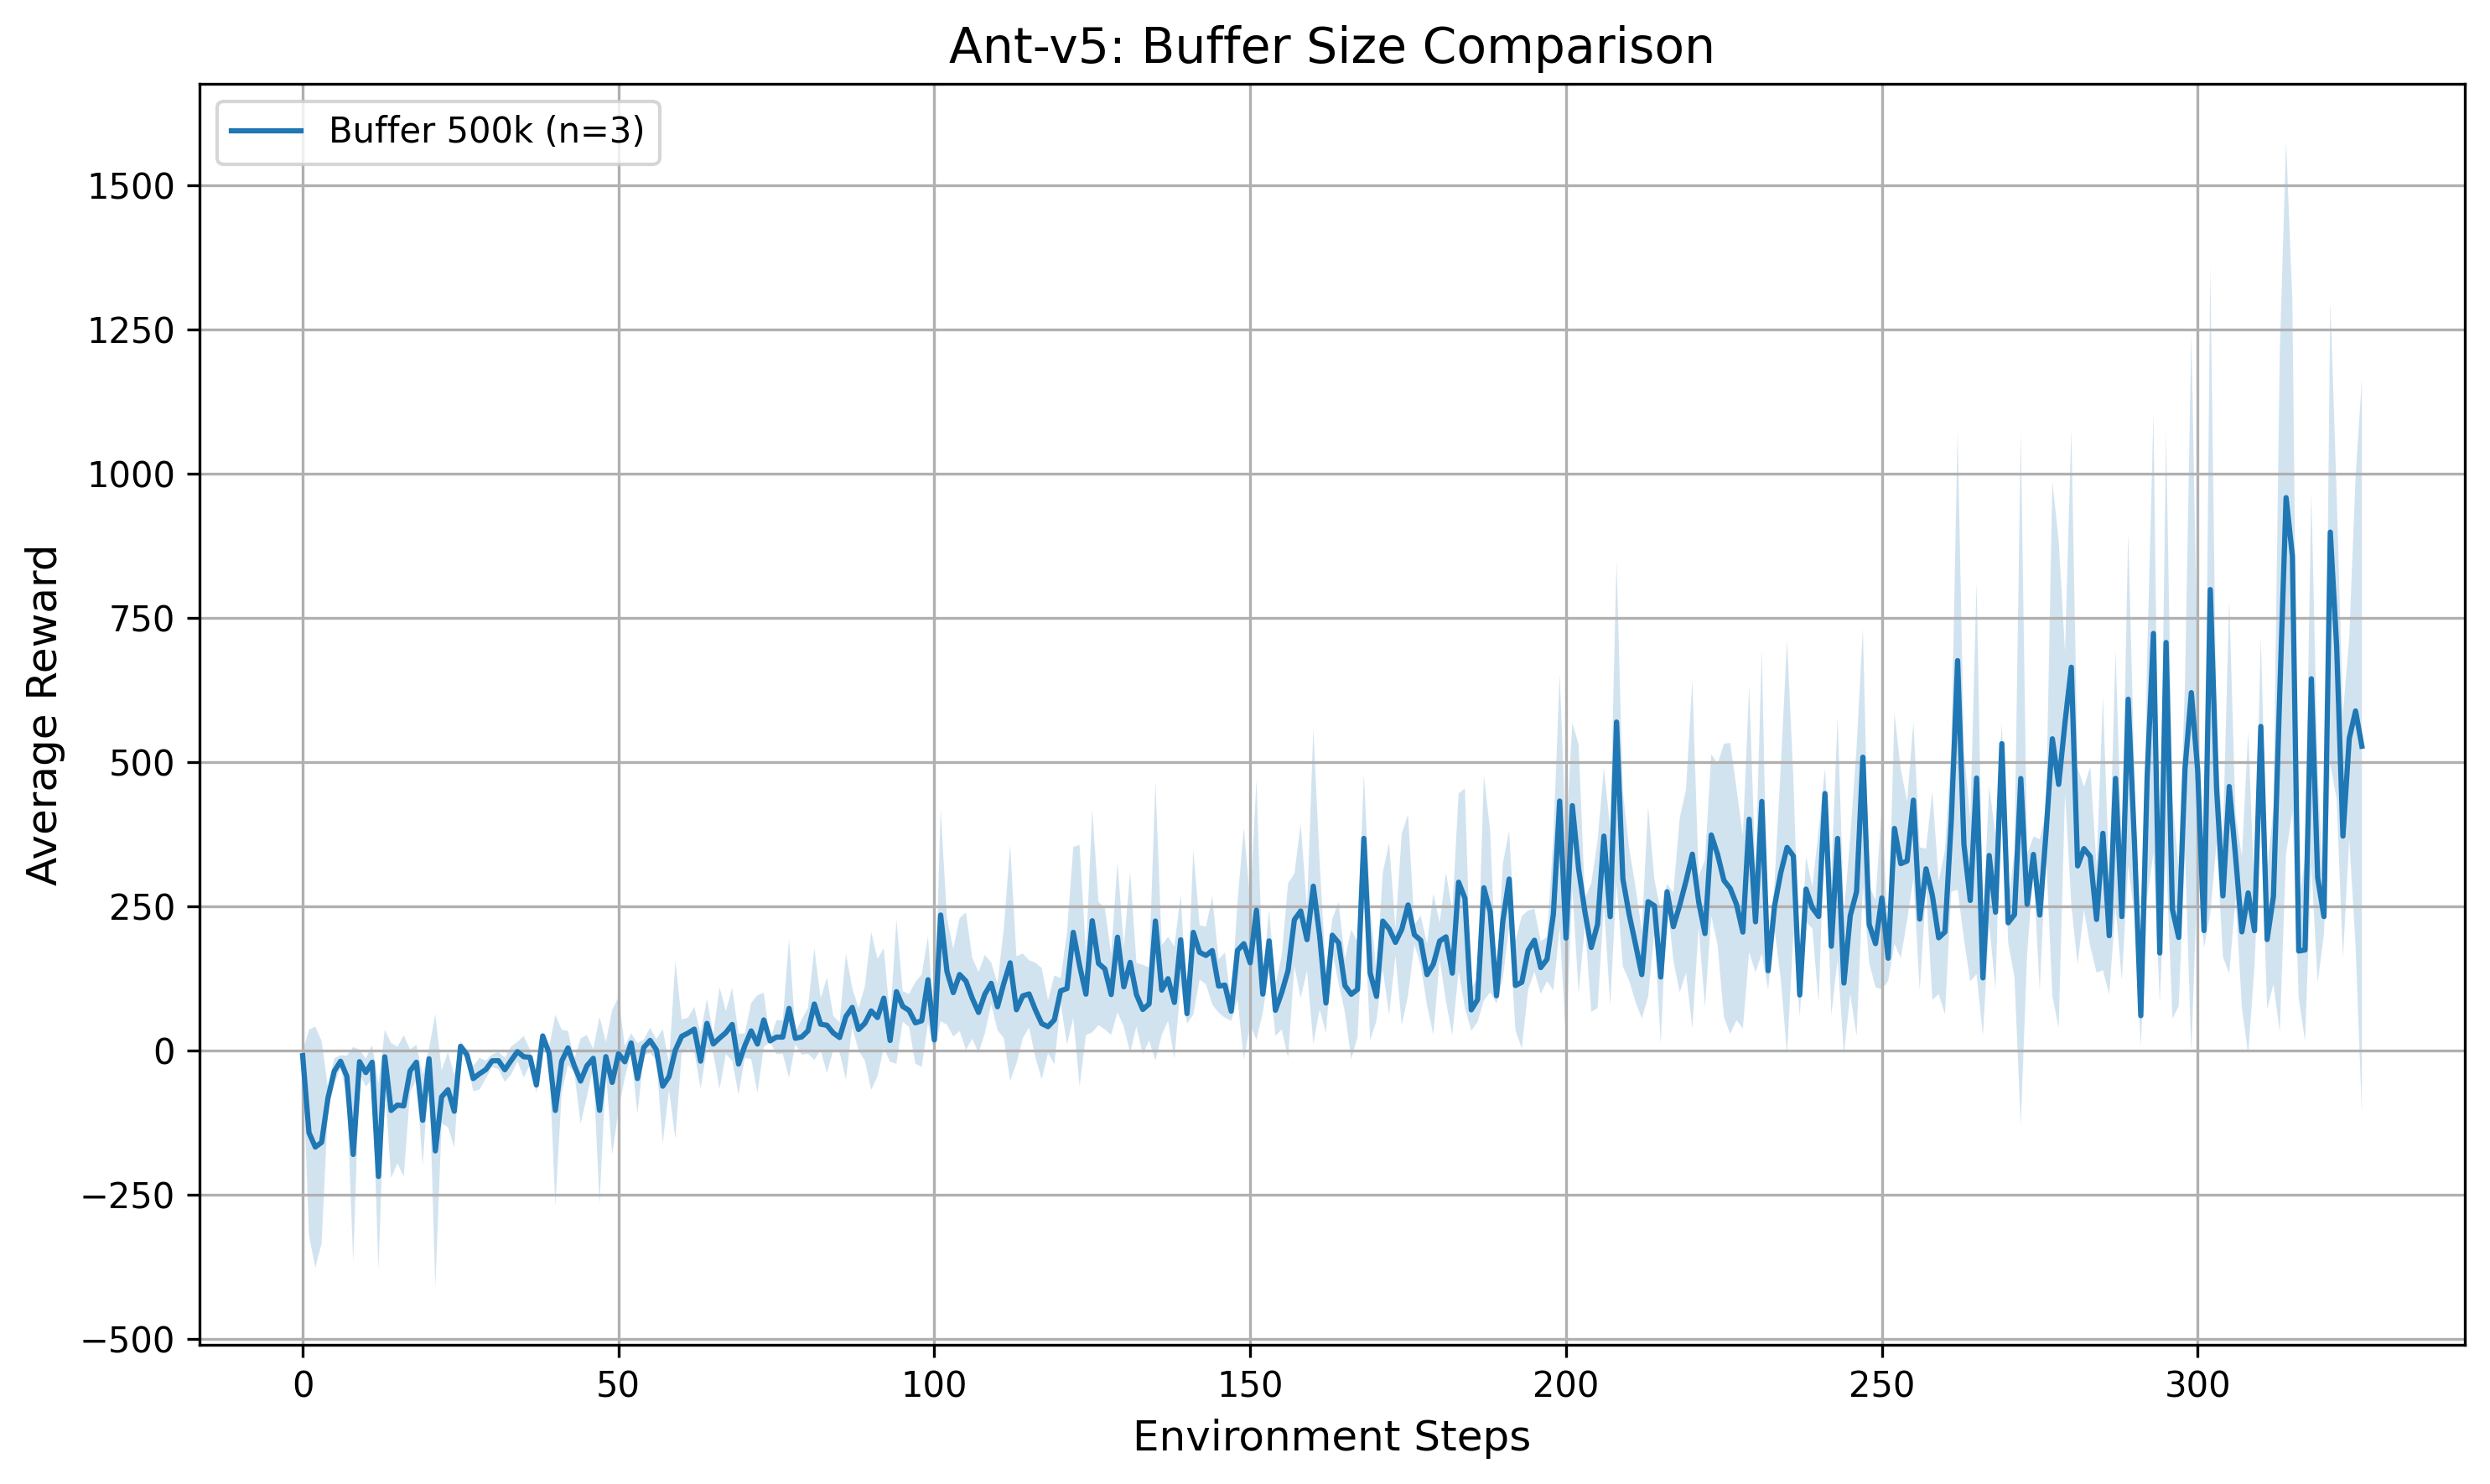
\includegraphics[width=0.7\textwidth]{figures/ant_buffer_comparison.png}
\caption{Learning curves for Ant-v5 with varying buffer sizes (n=3 seeds).}
\end{figure}

\textbf{Batch Size Comparison:}

\begin{figure}[H]
\centering
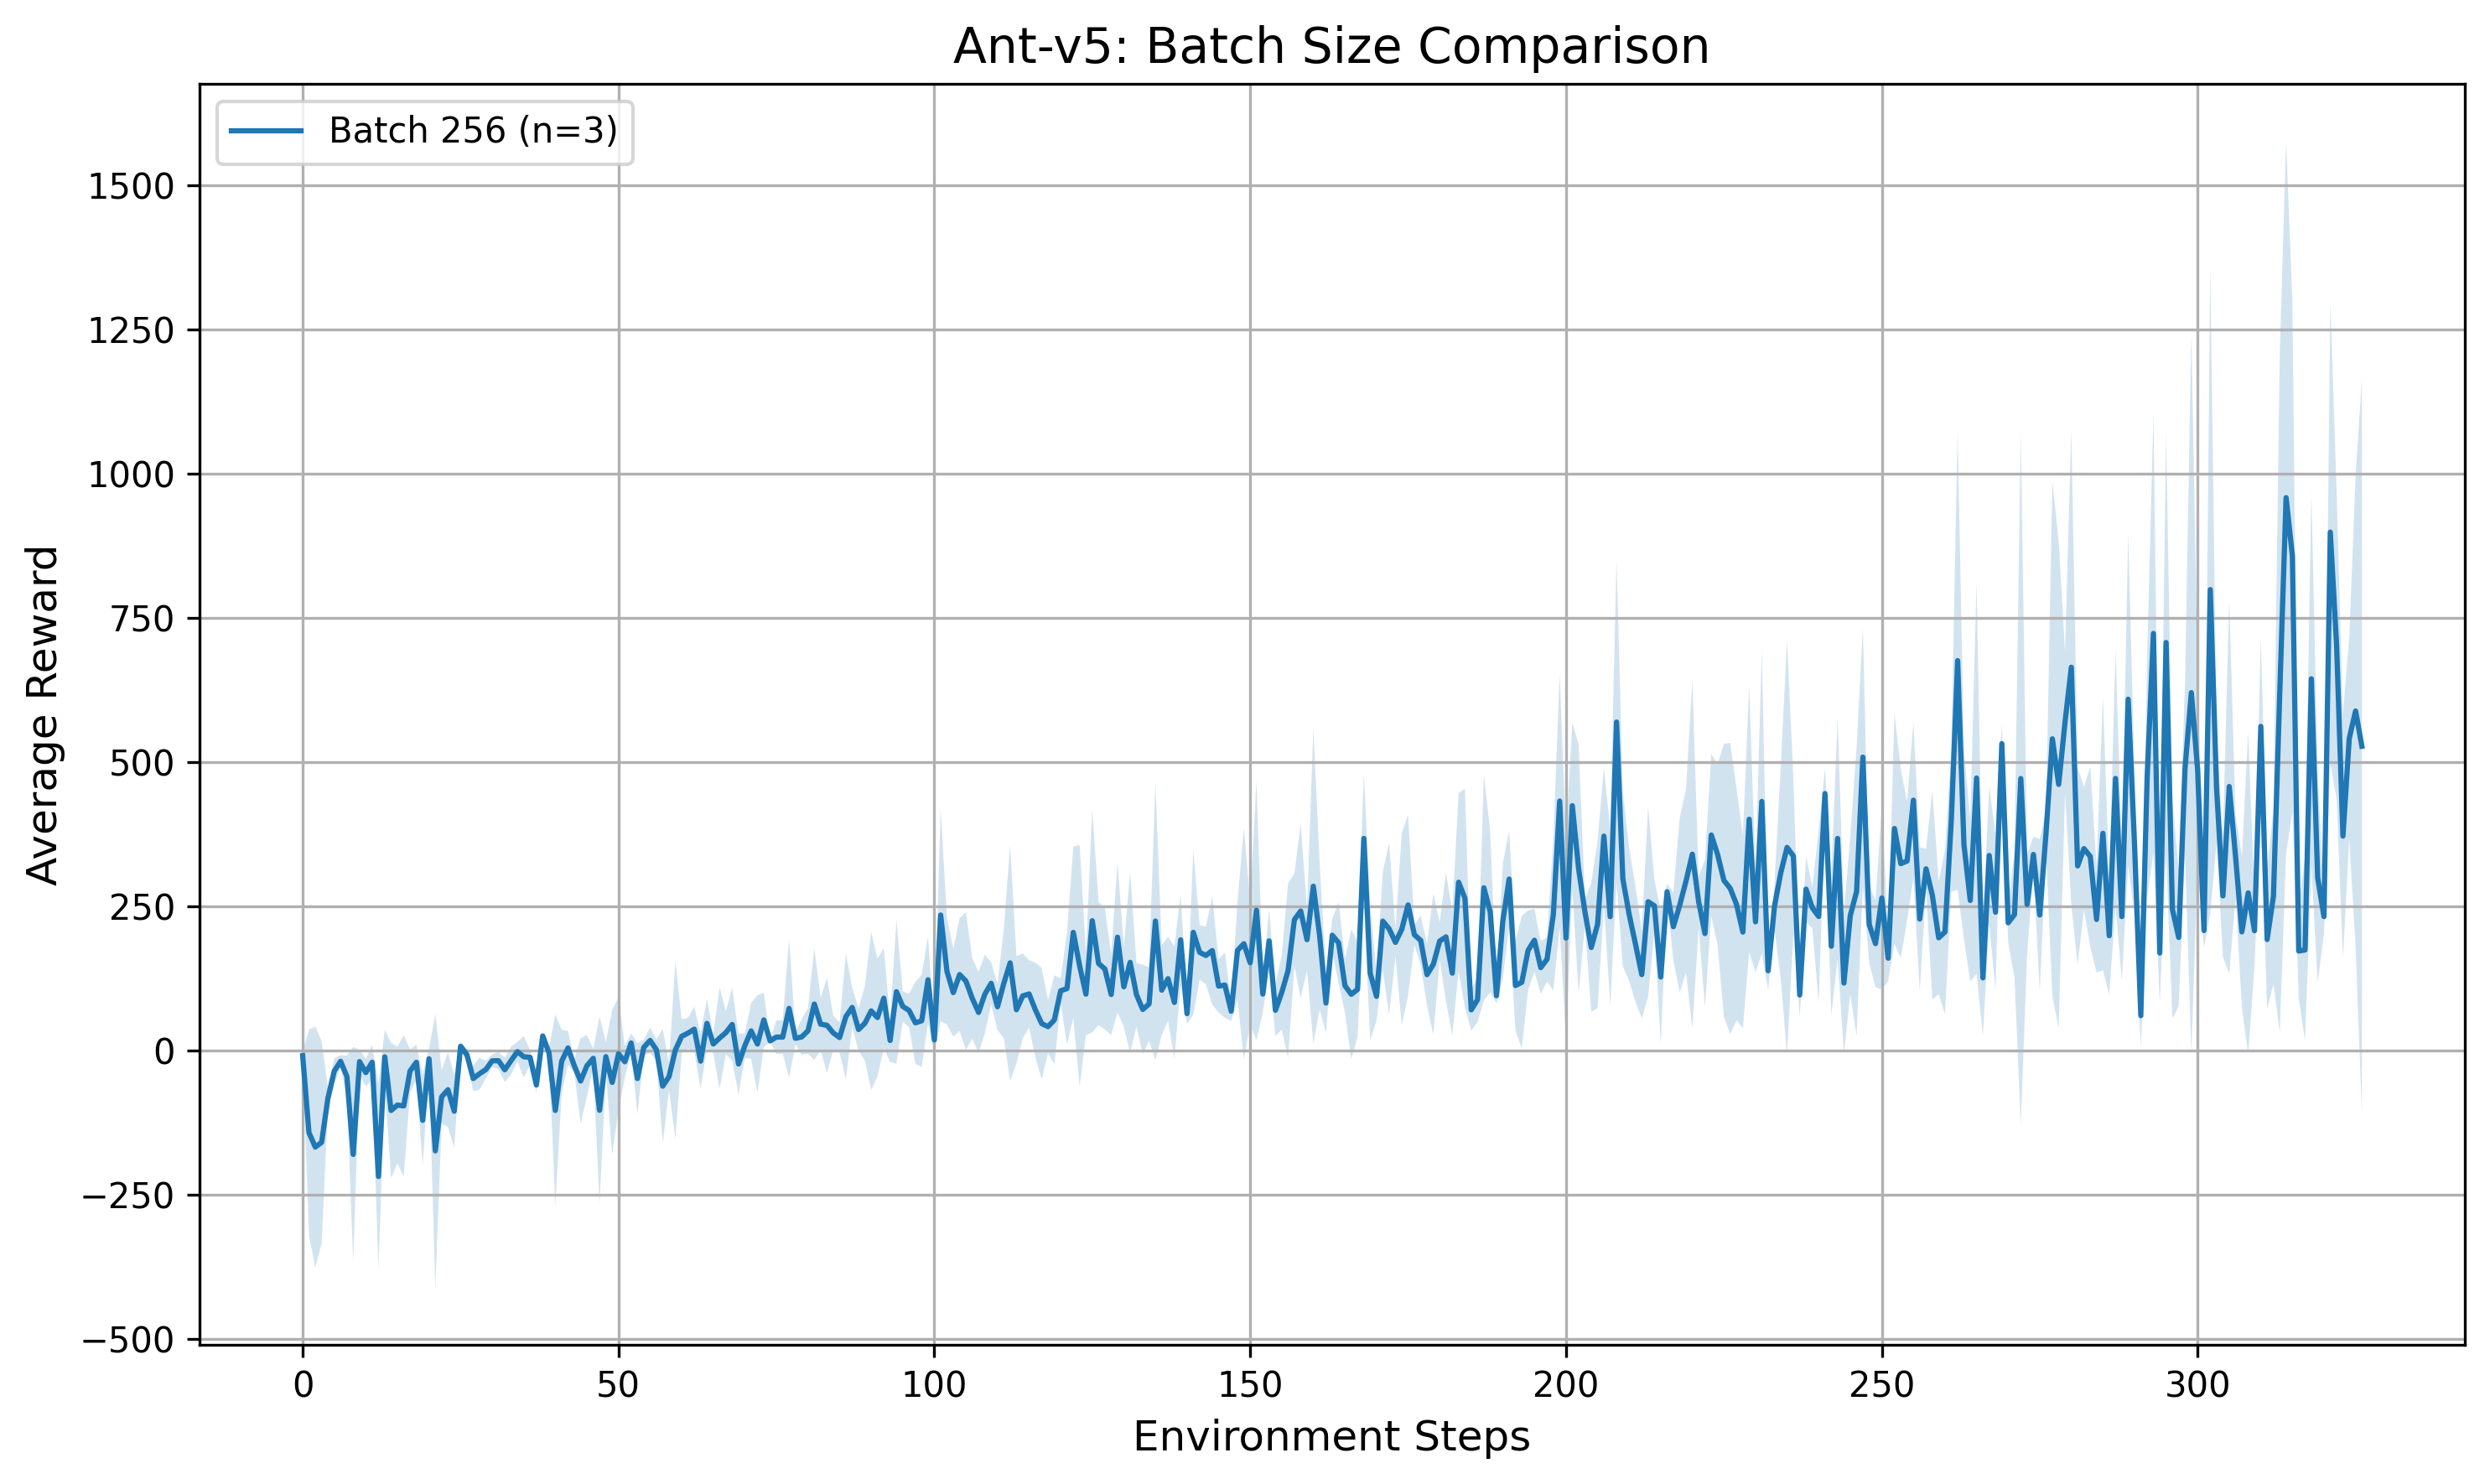
\includegraphics[width=0.7\textwidth]{figures/ant_batch_comparison.png}
\caption{Learning curves for Ant-v5 with varying batch sizes (n=3 seeds).}
\end{figure}

\textbf{Seed Variation:}

\begin{figure}[H]
\centering
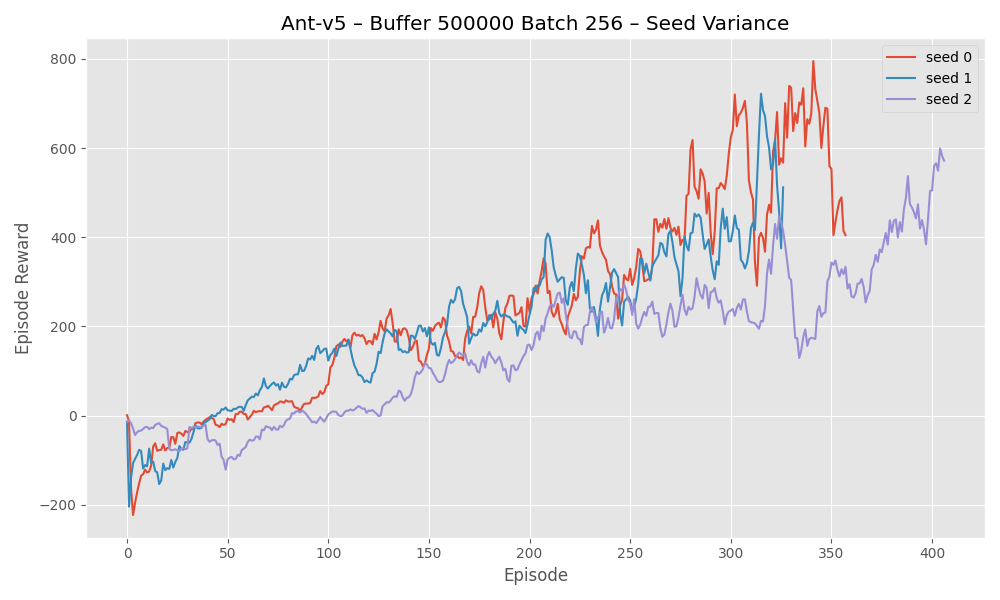
\includegraphics[width=0.7\textwidth]{figures/ant_seed_variance.png}
\caption{Seed variation for Ant-v5 across multiple runs (n=3 seeds).}
\end{figure}

\subsection{AntMaze (Placeholder)}

\begin{figure}[H]
\centering
\fbox{\parbox[c][5cm][c]{0.7\textwidth}{AntMaze Placeholder}}
\caption{AntMaze learning curves (placeholder).}
\end{figure}

\subsection{Walker2d (Placeholder)}

\begin{figure}[H]
\centering
\fbox{\parbox[c][5cm][c]{0.7\textwidth}{Walker2d Placeholder}}
\caption{Walker2d learning curves (placeholder).}
\end{figure}

\subsection{Evaluation Table}

\begin{figure}[H]
\centering
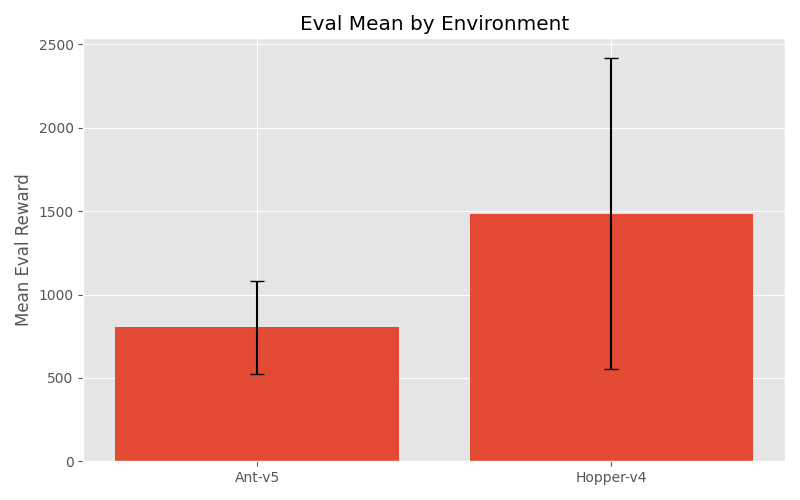
\includegraphics[width=0.7\textwidth]{figures/ant_vs_hopper_eval.png}
\caption{Comparison of mean and standard deviation of rewards across Hopper-v4 and Ant-v5 environments.}
\end{figure}

\begin{table}[H]
\centering
\begin{tabular}{l l l l l}
\toprule
Environment & Buffer & Batch & Mean Reward & Std Reward \\
\midrule
Ant-v5 & 500000 & 256 & 804.38 & 379.62 \\
Hopper-v4 & 50000 & 64 & 58.70 & 7.65 \\
Hopper-v4 & 300000 & 256 & 765.29 & 75.64 \\
Hopper-v4 & 500000 & 128 & 1461.51 & 329.18 \\
Hopper-v4 & 500000 & 256 & 2151.49 & 647.69 \\
Hopper-v4 & 500000 & 512 & 1583.25 & 369.99 \\
\bottomrule
\end{tabular}
\caption{Evaluation results aggregated across seeds for each environment, buffer size, and batch size.}
\end{table}

\section{Conclusion}
This project demonstrates that SAC performance improves with:

\begin{itemize}
    \item Pre-collected datasets in the replay buffer.
    \item Larger buffer sizes and moderate batch sizes.
    \item Multiple seeds for reliable evaluation.
\end{itemize}

\textbf{Limitations:}
\begin{itemize}
    \item Limited number of environments (Hopper, Ant-v5; AntMaze and Walker placeholders).
    \item Fewer seeds for some experiments due to computational constraints.
    \item Only SAC evaluated; future work could compare additional RL algorithms.
\end{itemize}

\textbf{Future Work:}
\begin{itemize}
    \item Extend experiments to more complex environments.
    \item Compare RLPD with other off-policy algorithms such as DDPG or TD3.
    \item Investigate the impact of dataset quality and diversity on learning outcomes.
\end{itemize}

\appendix
\section{References}
\begin{itemize}
    \item Ball, P. J., Smith, L., Kostrikov, I., \& Levine, S. (2023). \textit{Efficient Online Reinforcement Learning with Offline Data}. \href{https://arxiv.org/abs/2302.02948}{arXiv:2302.02948}
    \item RLPD GitHub Repository: \href{https://github.com/ikostrikov/rlpd}{https://github.com/ikostrikov/rlpd}
\end{itemize}

\end{document}
